\documentclass[../../main.tex]{subfiles}

\begin{document}

    Die aufgenommenen Spektren für angelegte Pumpströme $(I_P)_1 = 400\si{\mA}$ und $(I_P)_2 = 550\si{\mA}$ sind in Abbildung \ref{fig:TransmissionOverTemperature400mA} und \ref{fig:TransmissionOverTemperature550mA} zu sehen. Als Transmissionsleistung $P_t$ in Abhängigkeit von dem gewählten Pumpstrom $(I_P)_i$ definieren wir $P_{t,i}:=P_t((I_P)_i)$ als temperaturabhängige Transmissionsleitung.

    \begin{figure}[H]
        \centering
        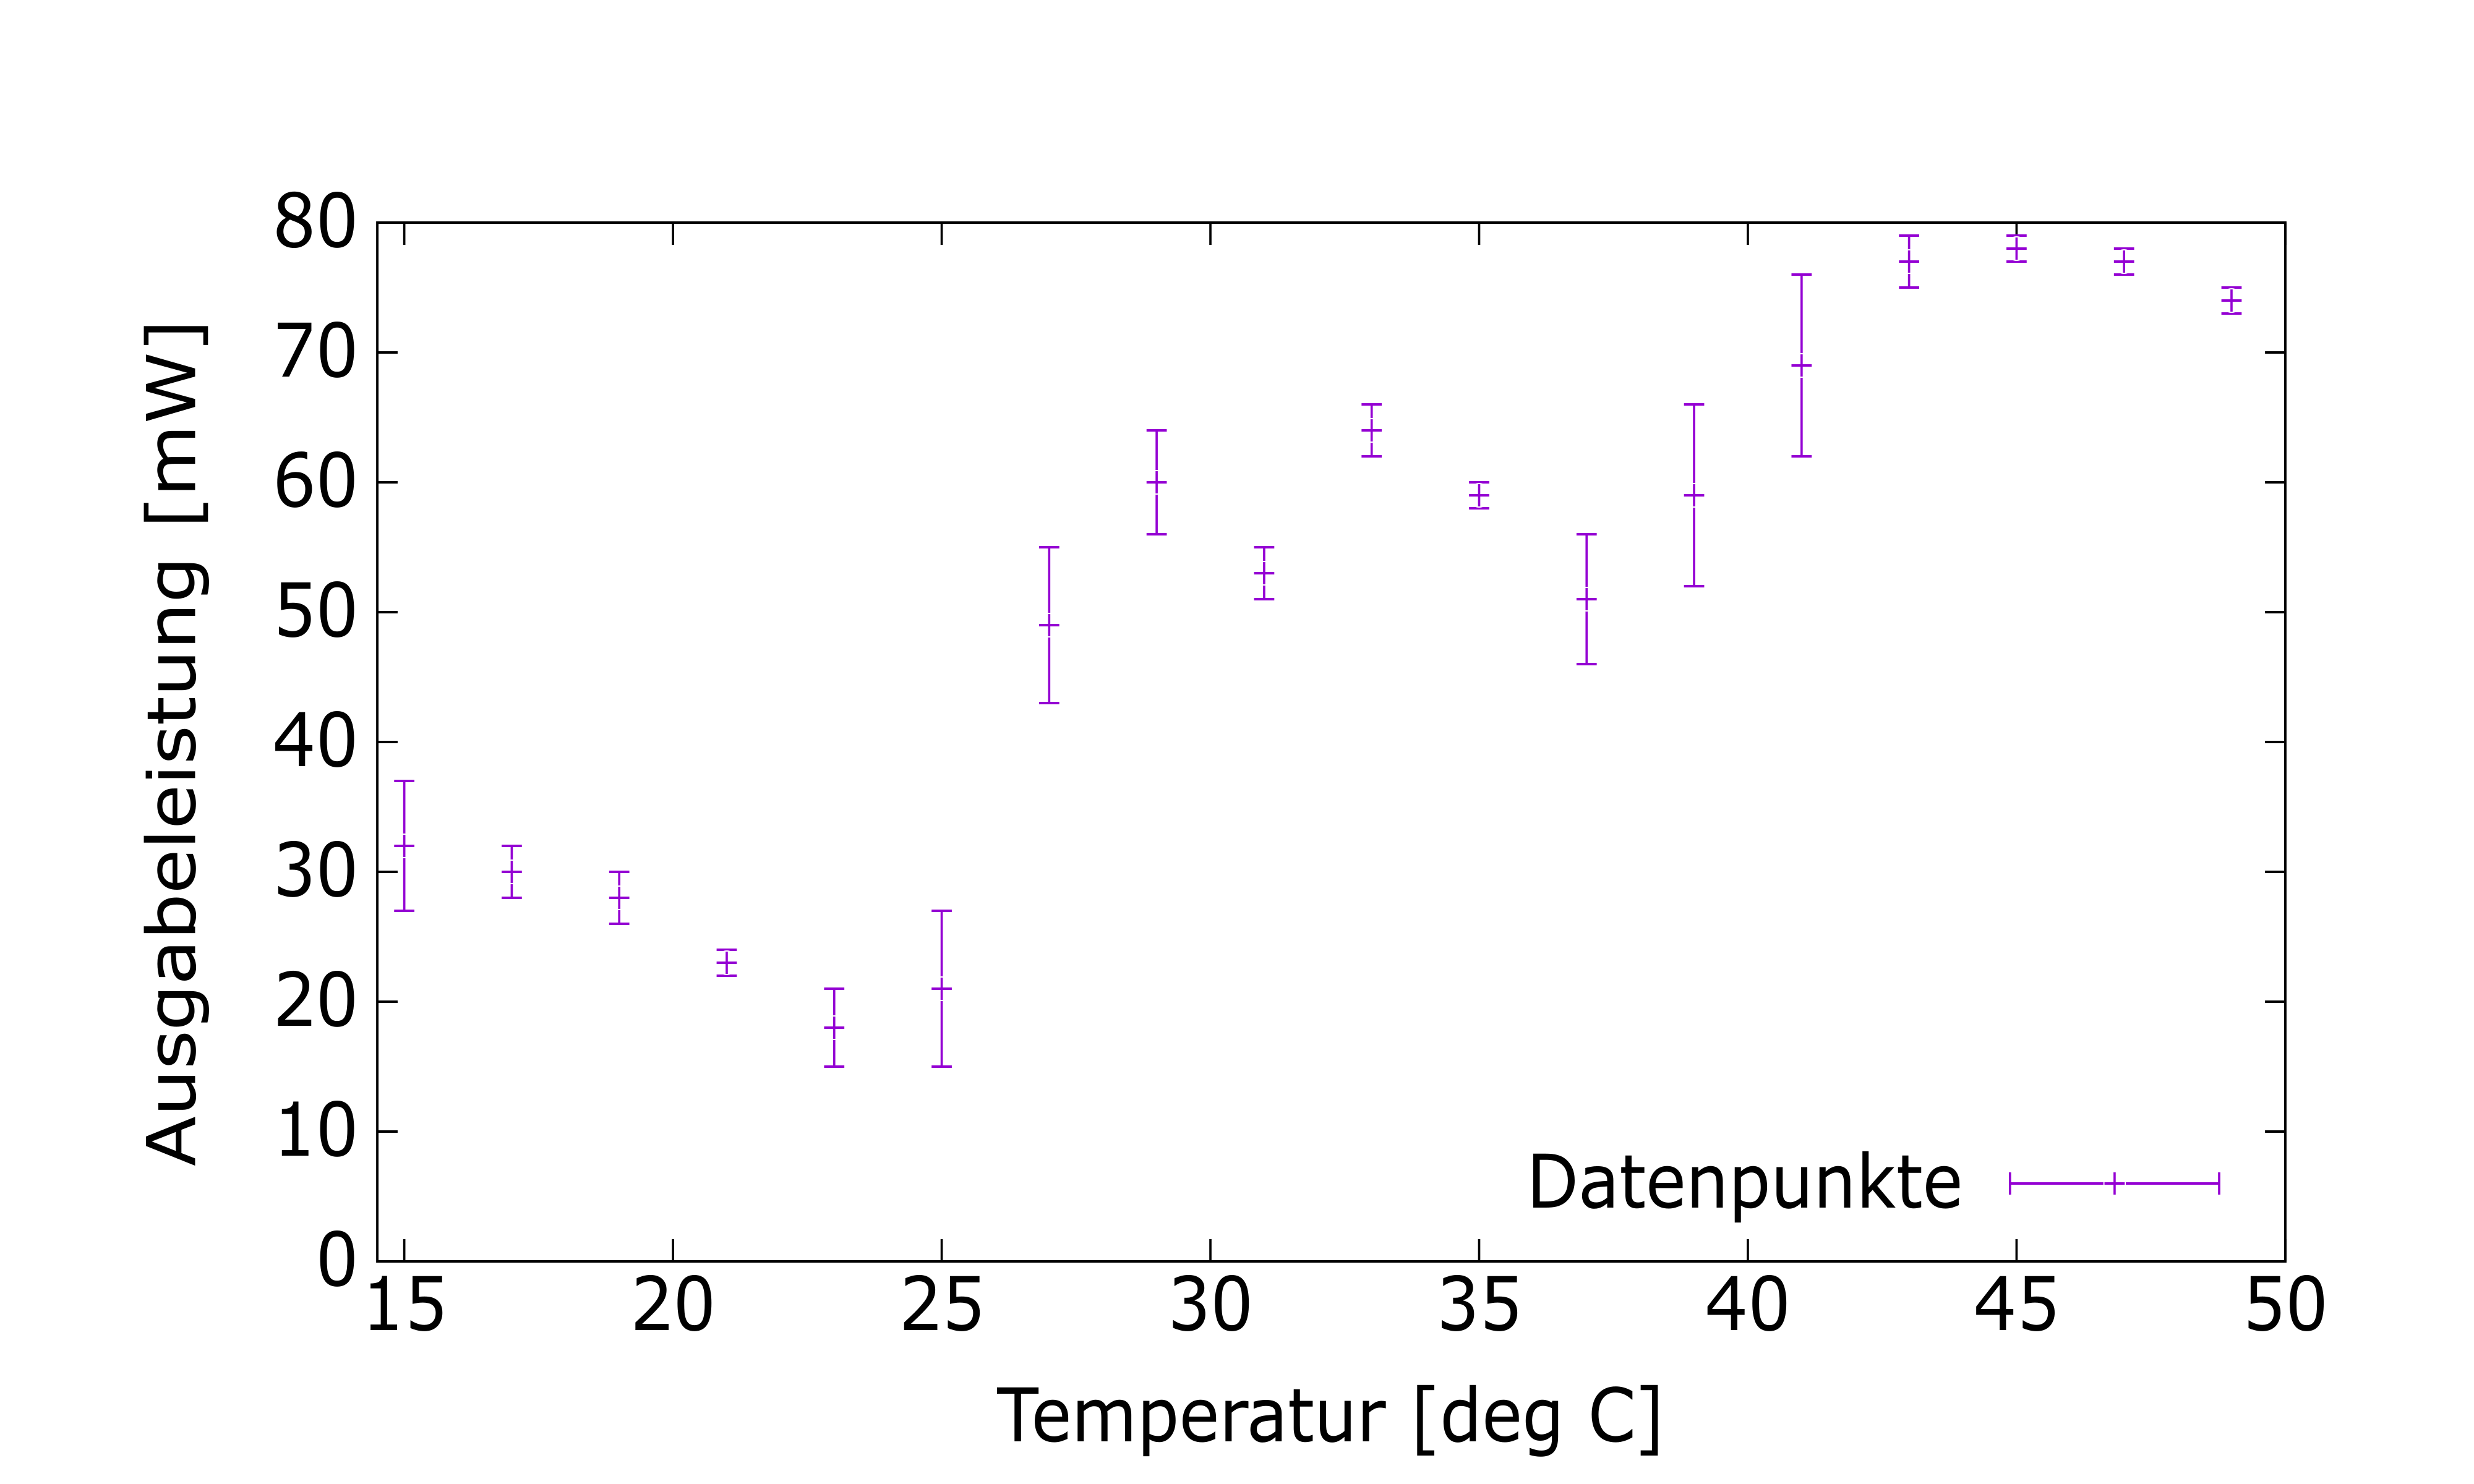
\includegraphics[width=11cm]{../../Bilddateien/1-1/TransmissionOverTemperature400mA.png}
        \caption{Die Transmissionsleistung $P_{t,i}$ als Funktion der Temperatur $T$ bei $(I_P)_1 = 400\si{\mA}$.}
        \label{fig:TransmissionOverTemperature400mA}
    \end{figure}

    \begin{figure}[H]
        \centering
        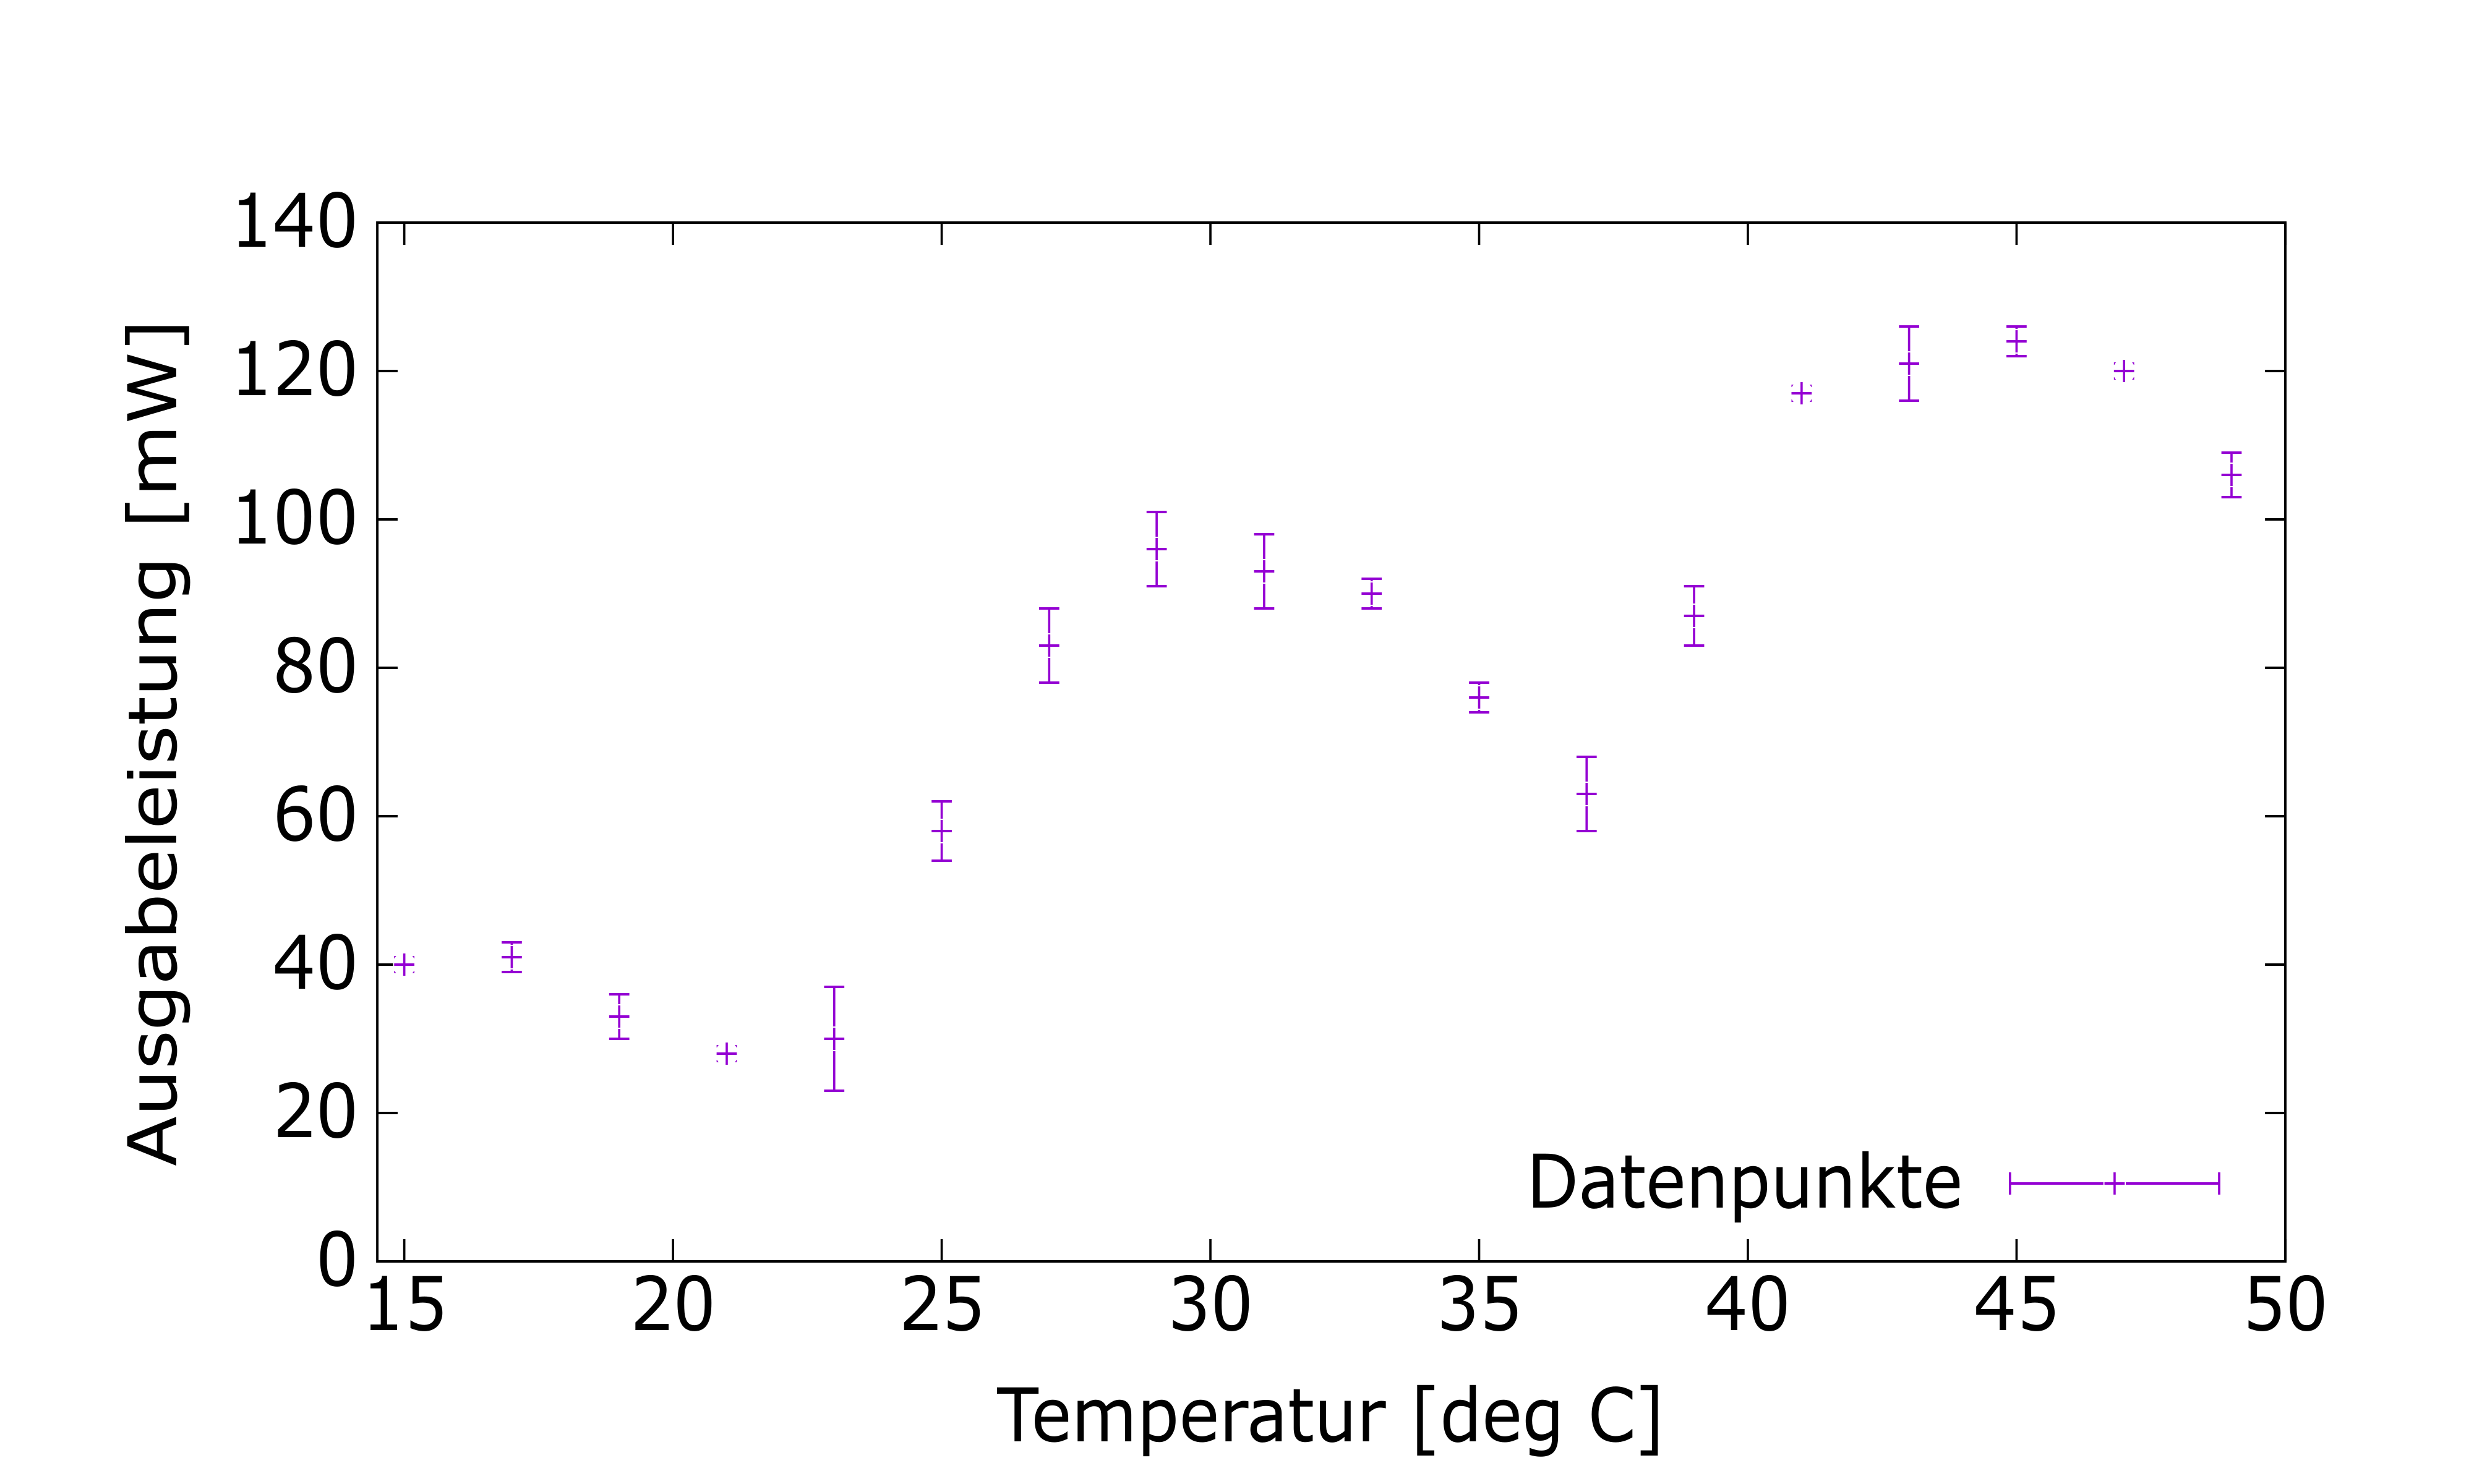
\includegraphics[width=11cm]{../../Bilddateien/1-1/TransmissionOverTemperature550mA.png}
        \caption{Die Transmissionsleistung $P_{t,i}$ als Funktion der Temperatur $T$ bei $(I_P)_2 = 550\si{\mA}$.}
        \label{fig:TransmissionOverTemperature550mA}
    \end{figure}
    Als Unsicherheiten verwenden wir hier empirisch bestimmte Unsicherheiten während der Aufnahme der Daten aufgrund der Fluktuationen der Messwerte.

    Die Minima der Graphen geben uns aufgrund geringster Transmission durch den Kristall die Pumplasertemperatur größter Absorbtion an, durch welche wir durch die jeweils konstante Pumpleistung auf die optimale Wellenlägen der Pumpstrahlung schließen können. In Tabelle \ref{tab:1-1:OptimaleParameterSpektrum} sind die optimalen Parameter für die Transmissionsfunktion $P_{t,i}$ durch in Form des minimierenden Arguments $T_{0,i}:=\text{argmin}(P_{t,i})$ aufgelistet. 
    \begin{table}[H]
        \centering
        \begin{tabular}{c|cc}
            \hline
            $(P_{\textit{an}})_i$ & $T_{0,i}$ & $P_{t,i}(T_{0,i})$ \\
            \hline\hline
            $(P_{\textit{an}})_1$ & $23.0(1)\si{\celsius}$ & $18(3)\si{\mW}$ \\
            $(P_{\textit{an}})_2$ & $21.0(1)\si{\celsius}$ & $28(1)\si{\mW}$ \\
        \end{tabular}
        \label{tab:1-1:OptimaleParameterSpektrum}
    \end{table}
    Wir können hier bereits eine Antiproportionalität zwischen der Anregungsleitung $P_{\textit{an}}$ und der zur Transmission optimalen Temperatur $T$ erkennen. Dies ist, wie wir in Kapitel \ref{subsec:1-2:KennlinieKonstanterDiodenlaserwellenlaenge} erkennen werden, ein valides experimentelles Ergebnis.
\end{document}